\documentclass[aspectratio=169,11pt]{beamer}

% common_setting.tex
% Shared preamble for the five PSPDE2026 workshop beamer decks (00-04).
% \input this right after \documentclass in each deck.
% Requires xelatex (fontspec/unicode-math need XeTeX or LuaTeX, not pdflatex).

% Fonts
\usepackage{fontspec}
\usepackage{unicode-math}
\setmainfont{Liberation Sans}
\setsansfont{Liberation Sans}
\setmonofont{Liberation Mono}[Scale=0.85]
\setmathfont{Latin Modern Math}

% Theme and colors
\usetheme{moloch}
\molochset{
  block=fill,
  progressbar=frametitle,
  sectionpage=progressbar,
}
\setbeamertemplate{page number in head/foot}[totalframenumber]

% Graphics
\usepackage{graphicx}
\graphicspath{{./figures/}}

% Tables
\usepackage{booktabs}
\usepackage{tabularx}

% Unnumbered captions without the "Figure:" label prefix
\usepackage{caption}
\captionsetup{labelformat=empty}

% Code listings
\usepackage{listings}
\usepackage{xcolor}
\definecolor{codebg}{RGB}{245,245,245}
% moloch's own accent colors, aliased under their original Metropolis names
\colorlet{mAlertFg}{mLightBrown}
\colorlet{mExampleFg}{mLightGreen}
\lstdefinestyle{python}{
  language=Python,
  basicstyle=\ttfamily\scriptsize,
  keywordstyle=\color{mAlertFg}\bfseries,
  commentstyle=\color{mExampleFg}\itshape,
  stringstyle=\color{mExampleFg!70!black},
  backgroundcolor=\color{codebg},
  rulecolor=\color{black!15},
  frame=single,
  breaklines=true,
  showstringspaces=false,
  columns=fullflexible,
  numbers=none
}
\lstdefinestyle{shell}{
  basicstyle=\ttfamily\scriptsize,
  backgroundcolor=\color{codebg},
  rulecolor=\color{black!15},
  frame=single,
  breaklines=true,
  columns=fullflexible
}


% Title information
\title[petropandas]{Processing Petrological Data with \texttt{petropandas}}
\subtitle{Block 3 --- Modern Workflow in Geology}
\author[O.\ Lexa]{Ondrej Lexa}
\institute[Charles University]{
  Institute of Petrology and Structural Geology (IPSG)\\
  Charles University, Prague, Czechia
}
\date{8 October 2026}

\begin{document}

\begin{frame}[plain]
  \titlepage
\end{frame}

\section{Motivation}

\begin{frame}{This Block (13:30--15:00)}
  \begin{block}{Objective}
    Turn a raw microprobe (EPMA) export into mineral formulas, end-members,
    a clean set of analyses and publication-ready charts --- in one notebook.
  \end{block}
  \vspace{0.3cm}
  \begin{enumerate}
    \item From Excel to \texttt{petropandas}
    \item Units: oxides $\rightarrow$ moles $\rightarrow$ cations
    \item Crystallochemical formulas \& end-members
    \item Data cleaning: totals and stoichiometry
    \item Charts \& export
  \end{enumerate}
  \vspace{0.2cm}
  \small Notebook: \texttt{notebooks/03\_petropandas.ipynb}
\end{frame}

\begin{frame}{Spreadsheets vs.\ Scripts}
  \begin{columns}[T]
    \begin{column}{0.48\textwidth}
      \begin{alertblock}{The usual Excel workflow}
        \small
        \begin{itemize}
          \item Copy-paste probe data into a recalculation sheet
          \item One sheet per mineral, formulas hidden in cells
          \item Delete ``bad'' rows by hand --- no record of why
          \item \texttt{Grt\_recalc\_v3\_FINAL2.xlsx}
        \end{itemize}
      \end{alertblock}
    \end{column}
    \begin{column}{0.48\textwidth}
      \begin{exampleblock}{A notebook pipeline}
        \small
        \begin{itemize}
          \item Raw export is \textbf{never edited}
          \item Every step (basis, Fe\textsuperscript{3+}, filter) is readable code
          \item Rejection criteria are explicit and re-runnable
          \item 10 or 10\,000 analyses --- same three lines
        \end{itemize}
      \end{exampleblock}
    \end{column}
  \end{columns}
\end{frame}

\begin{frame}{What is \texttt{petropandas}?}
  \begin{block}{In one sentence}
    A \textbf{pandas-accessor library}: oxide wt\% $\rightarrow$ moles
    $\rightarrow$ APFU $\rightarrow$ site-allocated formula
    $\rightarrow$ end-members, plus QC, bulk-rock helpers and plotting.
  \end{block}
  \vspace{0.3cm}
  \begin{center}
    \small
    \begin{tabular}{ll}
      \toprule
      \textbf{Accessor} & \textbf{Purpose} \\
      \midrule
      \texttt{df.oxides} & recognise \& clean oxide wt\% columns, filter rows \\
      \texttt{df.moles} / \texttt{df.cations} & wt\% $\leftrightarrow$ moles $\leftrightarrow$ APFU \\
      \texttt{df.mineral} & structural formulas, end-members, stoichiometry QC \\
      \texttt{df.bulk} & whole-rock: CIPW norm, ratios, THERMOCALC/MAGEMin input \\
      plotting & \texttt{ScatterPlot}, \texttt{TernaryPlot}, \texttt{ProfilePlot} \\
      \bottomrule
    \end{tabular}
  \end{center}
  \vspace{0.2cm}
  \centering No new file format, no new data structure --- just a \texttt{DataFrame}.
\end{frame}

\section{From Excel to petropandas}

\begin{frame}[fragile]{Loading an Instrument Export}
  \begin{columns}[T]
    \begin{column}{0.55\textwidth}
      \begin{lstlisting}[style=python]
from petropandas import pd, Grt, Fsp, Bt, Ms

df = pd.read_excel("data/epma_export.xlsx",
                   sheet_name="Spots")
df.oxides()          # only oxide columns

# mineral is hidden in the comment: S12_grt_03
df["Mineral"] = (df["Comment"]
                 .str.split("_").str[1])
grt = df.oxides.select("grt", on="Mineral")
      \end{lstlisting}
    \end{column}
    \begin{column}{0.42\textwidth}
      \small
      \begin{itemize}
        \item Plain \texttt{pd.read\_excel} / \texttt{read\_csv} --- no special reader
        \item Column names parsed as formulas; \texttt{Point}, \texttt{Comment}, \texttt{Total} ignored
        \item Vendor variants mapped automatically: \texttt{FeO*}, \texttt{FeOT}, \texttt{FeO tot} $\rightarrow$ \texttt{FeO}; \texttt{H2O+} $\rightarrow$ \texttt{H2O}
        \item \texttt{.select()} takes a substring, a list or a boolean mask
      \end{itemize}
    \end{column}
  \end{columns}
\end{frame}

\begin{frame}[fragile]{Units: Oxides $\rightarrow$ Moles $\rightarrow$ Cations}
  \begin{lstlisting}[style=python]
grt.oxides()                     # wt%
grt.moles()                      # molar proportions
apfu = grt.cations(n_oxygens=12) # atoms per formula unit, 12 O basis
apfu.attrs["petro_units"]        # 'apfu' - unit is tracked
apfu.oxides()                    # ... and conversions are reversible

apfu.cations.calc({"XMg":   "Mg{2+} / (Mg{2+} + Fe{2+})",
                   "Xsite": "Fe{2+} + Mg{2+} + Ca{2+} + Mn{2+}"})
  \end{lstlisting}
  \vspace{0.2cm}
  \small
  \begin{itemize}
    \item Ions are named with their charge: \texttt{Si\{4+\}}, \texttt{Fe\{2+\}}, \texttt{Na\{+\}}
    \item \texttt{df.cations(n\_cations=5)} for a cation-normalised basis (e.g.\ feldspar)
  \end{itemize}
\end{frame}

\section{Crystallochemical Formulas}

\begin{frame}[fragile]{Mineral Formulas and End-Members}
  \begin{lstlisting}[style=python]
grt.mineral.apfu(Grt)              # APFU incl. Fe3+/Fe2+ split (Droop 1987)
grt.mineral.site_allocations(Grt)  # structural formula: (site, cation) columns
grt.mineral.end_members(Grt)       # Prp, Alm, Sps, Grs, Adr, Uvr  (%)

pl.mineral.end_members(Fsp)        # An, Ab, Or
bt.mineral.end_members(Bt)         # Phl, Ann, Eas, Sid, Dioct
  \end{lstlisting}
  \vspace{0.2cm}
  \begin{block}{The pattern}
    Same three calls for every mineral --- only the \textbf{mineral object}
    changes. It carries the oxygen basis, ideal cation sum, Fe\textsuperscript{3+}
    method, site scheme and end-member set.
  \end{block}
\end{frame}

\begin{frame}{16 Built-in Mineral Definitions}
  \centering
  \footnotesize
  \begin{tabularx}{\textwidth}{lllcX}
    \toprule
    \textbf{Mineral} & \textbf{Object} & \textbf{O basis} & \textbf{Fe\textsuperscript{3+}} & \textbf{End-members} \\
    \midrule
    Garnet & \texttt{Grt} & 12 & Droop & Prp, Alm, Sps, Grs, \ldots \\
    Feldspar & \texttt{Fsp} & 8 & --- & An, Ab, Or \\
    Clinopyroxene & \texttt{Cpx} & 6 & Droop & Jd, Ae, Wo, En, Fs \\
    Orthopyroxene & \texttt{Opx} & 6 & Droop & MgTs, Wo, En, Fs \\
    Muscovite / Biotite & \texttt{Ms} / \texttt{Bt} & 11 & --- & Ms, Pg, Cel, \ldots{} / Phl, Ann, Sid, \ldots \\
    Amphibole & \texttt{Amp} & 23 & Schumacher & 13 end-members (Tr, Prg, Glau, \ldots) \\
    Chlorite & \texttt{Chl} & 14\textsuperscript{*} & --- & Clin, Cham, Pnn, Sud, \ldots \\
    Epidote / Titanite & \texttt{Ep} / \texttt{Ttn} & 12.5 / 5 & all Fe\textsuperscript{3+} & Czo, Ep, \ldots{} / Ttn, Al-Ttn, \ldots \\
    St, Cld, Crd & \texttt{St}, \texttt{Cld}, \texttt{Crd} & 48, 12, 18 & & \\
    Ilmenite, Spinel & \texttt{Ilm}, \texttt{Spl} & 3, 4 & Droop & \\
    \bottomrule
  \end{tabularx}

  \vspace{0.2cm}
  \raggedright
  \scriptsize \textsuperscript{*}28-charge normalisation. \texttt{from petropandas import mdb; mdb.all()} lists them all;
  \texttt{GrtFe3} estimates Fe\textsuperscript{3+} by matrix inversion.
  THERMOCALC a--x models are in \texttt{petropandas.hpxeos}.
\end{frame}

\section{Data Cleaning}

\begin{frame}[fragile]{Two Independent Quality Checks}
  \begin{columns}[T]
    \begin{column}{0.5\textwidth}
      \small
      \textbf{1. Analytical total}\\
      $\approx$ 98.5--101.5 wt\% anhydrous,\\ $\approx$ 94--97 wt\% micas
      \vspace{0.2cm}

      \textbf{2. Stoichiometry}\\
      \texttt{check\_stoichiometry(M)} scores each criterion 0--1:
      \texttt{analytical\_total}, \texttt{cation\_deviation},
      \texttt{charge\_balance}, \texttt{site\_vacancies},
      \texttt{leftover\_cations}, \ldots\\
      \texttt{stoichiometry\_quality(M)} = one number
    \end{column}
    \begin{column}{0.5\textwidth}
      \begin{lstlisting}[style=python]
def clean(data, mineral,
          total=(98.5, 101.5),
          min_quality=0.97):
    tot = data.oxides().sum(axis=1)
    q = data.mineral\
        .stoichiometry_quality(mineral)
    ok = (tot.between(*total)
          & (q >= min_quality))
    return data.oxides.select(ok)

grt_ok = clean(grt, Grt)
bt_ok = clean(bt, Bt, total=(94, 97.5))
      \end{lstlisting}
    \end{column}
  \end{columns}
\end{frame}

\begin{frame}{Why Both Checks?}
  \begin{columns}[T]
    \begin{column}{0.5\textwidth}
      \begin{alertblock}{Low total, perfect formula}
        \small
        A spot on a crack gives a total of $\sim$88 wt\% --- but all oxides are
        reduced \emph{proportionally}, so the recalculated formula is
        \textbf{perfect}. Only the total catches it.
      \end{alertblock}
    \end{column}
    \begin{column}{0.5\textwidth}
      \begin{alertblock}{Good total, wrong formula}
        \small
        A garnet spot partly on a plagioclase inclusion has a perfect total
        ($\sim$99.7 wt\%), but the cation sum and site occupancy are off.
        Only stoichiometry catches it.
      \end{alertblock}
    \end{column}
  \end{columns}
  \vspace{0.4cm}
  \begin{block}{Rule}
    Combine the two, keep the thresholds in code, and \textbf{print what was
    rejected} --- your filter becomes part of the methods section.
  \end{block}
\end{frame}

\section{Charts \& Export}

\begin{frame}[fragile]{Three Plot Classes, One Pattern}
  \begin{columns}[T]
    \begin{column}{0.55\textwidth}
      \begin{lstlisting}[style=python]
from petropandas import (TernaryPlot,
    ScatterPlot, ProfilePlot)

t = TernaryPlot("An", "Ab", "Or")
t.add(pl_ok.mineral.end_members(Fsp),
      label="S12 plagioclase")
t.show()

s = ScatterPlot("Si{4+}",
    "Fe{2+} / (Fe{2+} + Mg{2+})")
s.add(bt_ok.mineral.apfu(Bt), label="Bt")
s.savefig("output/micas.pdf")
      \end{lstlisting}
    \end{column}
    \begin{column}{0.42\textwidth}
      \begin{figure}
        \centering
        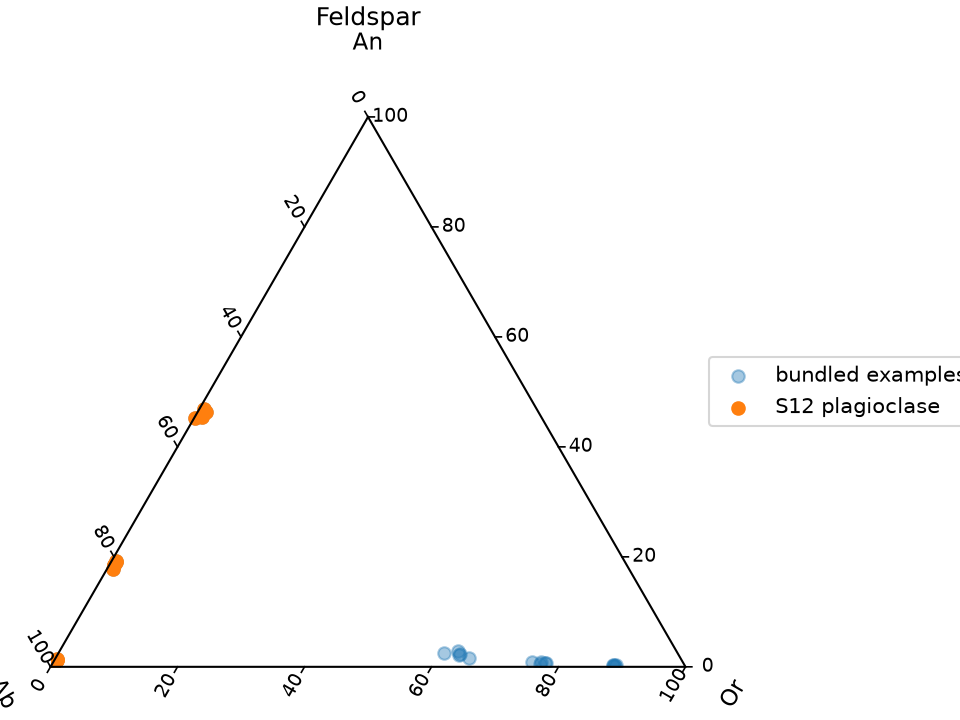
\includegraphics[width=\textwidth,height=0.6\textheight,keepaspectratio]{pp_fsp_ternary.png}
      \end{figure}
      \small Axes are \textbf{expressions} --- no helper columns needed.
    \end{column}
  \end{columns}
\end{frame}

\begin{frame}{Examples from the Notebook}
  \begin{columns}[T]
    \begin{column}{0.5\textwidth}
      \begin{figure}
        \centering
        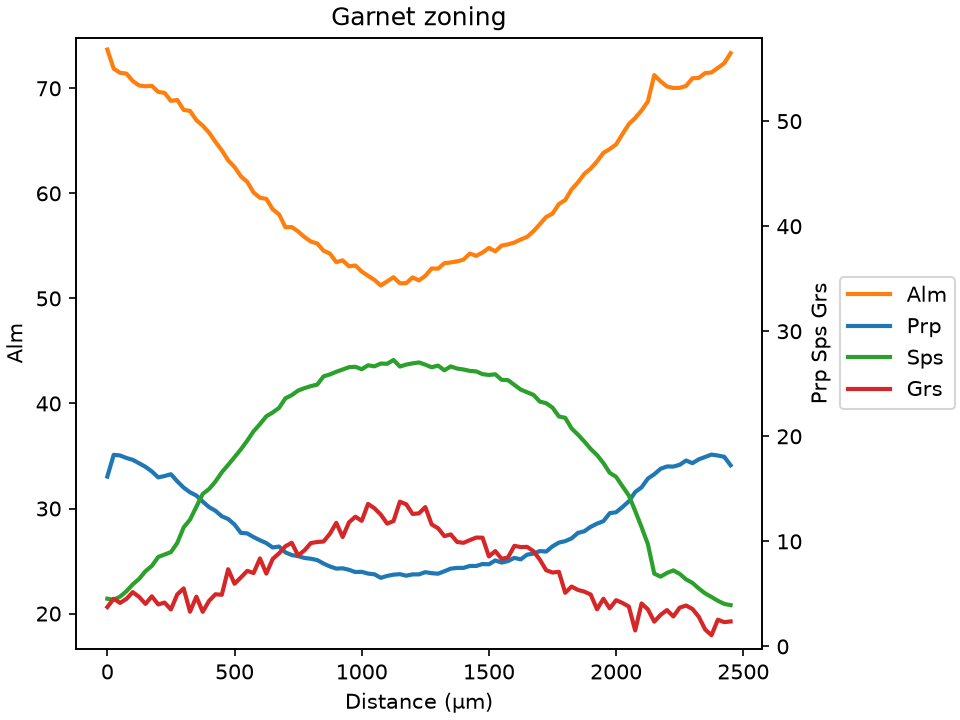
\includegraphics[width=\textwidth,height=0.62\textheight,keepaspectratio]{pp_grt_profile.png}
        \caption*{\footnotesize \texttt{ProfilePlot}: garnet traverse, \texttt{split="auto"}}
      \end{figure}
    \end{column}
    \begin{column}{0.5\textwidth}
      \begin{figure}
        \centering
        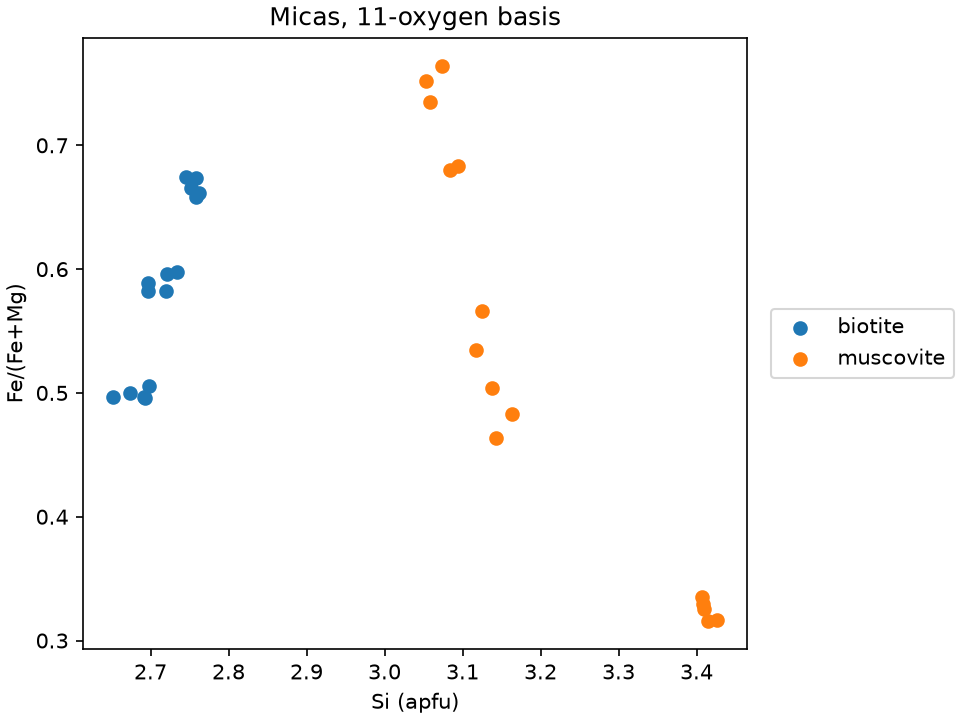
\includegraphics[width=\textwidth,height=0.62\textheight,keepaspectratio]{pp_mica_scatter.png}
        \caption*{\footnotesize \texttt{ScatterPlot}: Si vs.\ Fe/(Fe+Mg) in micas}
      \end{figure}
    \end{column}
  \end{columns}
\end{frame}

\begin{frame}[fragile]{Exporting Results}
  \begin{lstlisting}[style=python]
with pd.ExcelWriter("output/S12_results.xlsx") as xls:
    grt_ok.mineral.apfu(Grt).round(4).to_excel(xls, sheet_name="Grt apfu")
    grt_ok.mineral.end_members(Grt).round(2).to_excel(xls, sheet_name="Grt end-members")
    pl_ok.mineral.end_members(Fsp).round(2).to_excel(xls, sheet_name="Pl end-members")

p.savefig("output/grt_profile.pdf")     # vector graphics: .pdf / .svg
  \end{lstlisting}
  \vspace{0.2cm}
  \small
  \begin{itemize}
    \item Results are ordinary DataFrames --- any pandas writer works
          (\texttt{to\_excel}, \texttt{to\_csv}, \texttt{to\_latex})
    \item Whole-rock data? \texttt{df.bulk.cipw()}, \texttt{.oxide\_ratios()},
          \texttt{.TCbulk()}, \texttt{.MAGEMin()}
  \end{itemize}
\end{frame}

\section{Hands-on}

\begin{frame}{Hands-on Exercise}
  \textbf{Muscovite analyses in \texttt{data/epma\_export.xlsx}} (notebook section 3.7)
  \begin{enumerate}
    \item Select the \texttt{ms} rows and recalculate them with \texttt{Ms}
    \item Clean them with \texttt{clean()} --- choose a sensible total window
          for a hydrous mineral
    \item End-members and Si (apfu): is there a phengite (celadonite) component?
    \item \texttt{ScatterPlot} of Si vs.\ Na/(Na+K), saved as SVG to \texttt{output/}
    \item \emph{Bonus:} mean matrix garnet vs.\ rim of the garnet profile
  \end{enumerate}
\end{frame}

\section{Recap}

\begin{frame}{Recap \& Resources}
  \begin{block}{Key takeaways}
    \begin{itemize}
      \item Raw export $\rightarrow$ APFU $\rightarrow$ end-members, all on a \texttt{DataFrame}
      \item One mineral object carries the whole recalculation recipe
      \item Filter on \textbf{total and stoichiometry}, and log what you reject
      \item Expression-based plots, vector output, Excel export
    \end{itemize}
  \end{block}
  \vspace{0.3cm}
  \textbf{Resources:} \texttt{github.com/ondrolexa/petropandas} (docs \& walkthrough notebook)
  \vspace{0.4cm}

  \centering \Large Next: Bring Your Own Data --- \texttt{04b\_byod\_epma.ipynb}
\end{frame}

\end{document}
